% This file was created by matlab2tikz.
%
%The latest updates can be retrieved from
%  http://www.mathworks.com/matlabcentral/fileexchange/22022-matlab2tikz-matlab2tikz
%where you can also make suggestions and rate matlab2tikz.
%

\definecolor{mycolor1}{rgb}{0.00000,0.44700,0.74100}%
\definecolor{mycolor2}{rgb}{0.85000,0.32500,0.09800}%
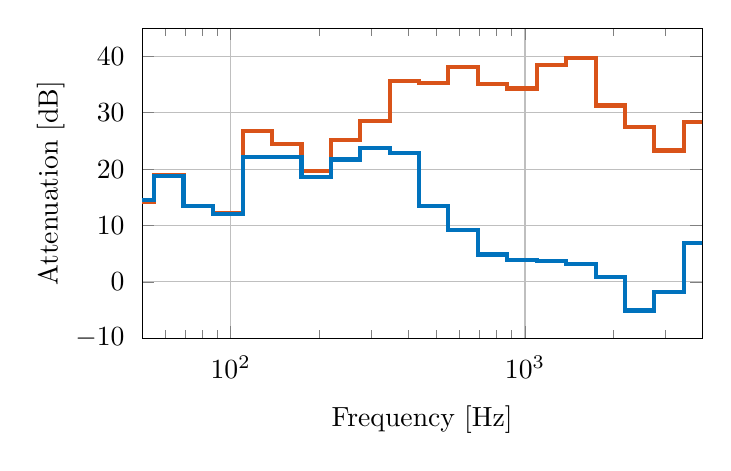
\begin{tikzpicture}

\begin{axis}[%
width=2.8in,
height=1.55in,
scale only axis,
%scaled y ticks = false,
xmode=log,
xmin=50,
xmax=4000,
xlabel={Frequency [Hz]},
xmajorgrids,
ymin=-10,
ymax=45,
ylabel style={yshift=-0.3em},
xlabel style={yshift=-0.3em},
ytick={-10,0,...,40},
%yticklabels={50,400,800,2000,4000},
ylabel={Attenuation [dB]},
ymajorgrids,
axis background/.style={fill=white},
title style={font=\bfseries},
xticklabel shift={.1cm},
yticklabel shift={.1cm}
%title={Comparison}
]
\addplot[const plot,color=mycolor2,solid,forget plot,thick, line width=1.5pt] plot table[row sep=crcr] {%
21.9	8.53\\
27.5	9.92\\
34.7	15\\
43.6	14.2\\
54.9	19\\
69.1	13.5\\
87.1	12.2\\
110	26.7\\
138	24.4\\
174	19.6\\
219	25.2\\
275	28.5\\
347	35.7\\
436	35.3\\
549	38.1\\
691	35.1\\
871	34.3\\
1.1e+03	38.5\\
1.38e+03	39.7\\
1.74e+03	31.3\\
2.19e+03	27.4\\
2.75e+03	23.3\\
3.47e+03	28.4\\
4.36e+03	24.1\\
5.49e+03	13.9\\
6.91e+03	10.2\\
8.71e+03	23.6\\
1.1e+04	19.1\\
1.38e+04	13.2\\
1.79e+04	2.94\\
};
\addplot[const plot,color=mycolor1,solid,forget plot,thick,line width=1.5pt] plot table[row sep=crcr] {%
21.9	8.7\\
27.5	10.1\\
34.7	15.2\\
43.6	14.5\\
54.9	18.8\\
69.1	13.4\\
87.1	12\\
110	22.1\\
138	22.2\\
174	18.6\\
219	21.7\\
275	23.7\\
347	22.8\\
436	13.5\\
549	9.13\\
691	4.85\\
871	3.85\\
1.1e+03	3.75\\
1.38e+03	3.18\\
1.74e+03	0.859\\
2.19e+03	-5.09\\
2.75e+03	-1.73\\
3.47e+03	6.95\\
4.36e+03	15.9\\
5.49e+03	6.78\\
6.91e+03	7.84\\
8.71e+03	24.8\\
1.1e+04	15\\
1.38e+04	13.8\\
1.79e+04	4.07\\
};
%% Difference
%\addplot[const plot,color=black,solid,forget plot,dashed,line width =1.5pt] plot table[row sep=crcr] {%
%	21.9	-0.173\\
%	27.5	-0.221\\
%	34.7	-0.25\\
%	43.6	-0.32\\
%	54.9	0.271\\
%	69.1	0.135\\
%	87.1	0.197\\
%	110	4.55\\
%	138	2.2\\
%	174	1.03\\
%	219	3.43\\
%	275	4.71\\
%	347	12.9\\
%	436	21.7\\
%	549	29\\
%	691	30.2\\
%	871	30.5\\
%	1.1e+03	34.7\\
%	1.38e+03	36.5\\
%	1.74e+03	30.4\\
%	2.19e+03	32.4\\
%	2.75e+03	25\\
%	3.47e+03	21.5\\
%	4.36e+03	8.12\\
%	5.49e+03	7.14\\
%	6.91e+03	2.4\\
%	8.71e+03	-1.21\\
%	1.1e+04	4.14\\
%	1.38e+04	-0.574\\
%	1.79e+04	-1.12\\
%};

\end{axis}
\end{tikzpicture}%